% !TEX root = ../../1-te.tex

\subsection{Module und Co.}
	Um euren Abschluss zu bekommen müsst ihr eine vordefinierte Menge von Modulen abdecken. Ein Modul besteht aus verschiedenen Bestandteilen.

\subsubsection{Vorlesung, Übung, etc.}
	\paragraph*{Vorlesung}
	Vorlesungen werden vor allen Studis abgehalten und befassen sich in erster Linie mit der theoretischen Herleitung des Stoffes. Solltest du in der Vorlesung einmal etwas nicht verstehen, so ist das nicht so tragisch. Vorlesungen an der Uni unterscheiden sich stark vom Unterricht an der Schule. Gehe nicht davon aus, Vorlesungsinhalte direkt zu verstehen. Plane eine gewisse Nachbearbeitungszeit für die Vorlesungen ein. In einer Vorlesung ist wegen der großen Teilnehmerzahl normalerweise kein Dialog mit dem oder der Vortragenden möglich. Aufgetretene Fragen können und sollten am besten direkt nach der Vorlesung oder sonst in einer Sprechstunde mit der oder dem Lehrenden geklärt werden.
	
	\paragraph*{Große Übung}
	Ergänzend gibt es die großen Übungen, auch Saalübungen genannt. Diese finden, wie die Vorlesung, vor dem gesamten Auditorium statt und sollen das erworbene, theoretische Wissen vertiefen und vor allem auch praktische, klausurbezogene Anwendungen aufzeigen. Die große Übung wird normalerweise von einer Mitarbeiterin oder einem Mitarbeiter gehalten. Sie sind bei  fachlichen Fragen kompetente Ansprechpartner/innen und meistens auch sehr hilfsbereit. Da sie  üblicherweise die Klausuren entwerfen, kann man bei genauem Hinhören in den großen Übungen oder im privaten Gespräch mit ihnen einiges über die Prüfung erfahren.

	\paragraph*{Kleine Übung, Seminargruppe}
	Als erstes eine Warnung: Kleine Übungen tauchen im Stundenplan nicht immer auf und werden leider nur in einigen Fächern angeboten. Der Begriff Seminargruppe ist synonym zu verstehen.
	
	In kleinen Übungen soll man selbst Aufgaben lösen. Dies geschieht unter Anleitung der HiWis (Hilfswissenschaftler/innen), welche meist Studierende höheren Semesters sind. Für die kleinen Übungen werden die Studis in etwa 20- bis 30-köpfige Gruppen aufgeteilt. Hierbei ist darauf zu achten, rechtzeitig zum Termin der Gruppeneinteilung zu erscheinen, um diese Veranstaltungen möglichst günstig im Stundenplan positionieren zu können. Der Termin wird meistens in der ersten Vorlesung bzw. großen Übung bekannt gegeben oder steht auf der jeweiligen Institutsseite. Aufgrund der geringen Teilnehmerzahlen ist in kleinen Übungen der Dialog mit der oder dem Vortragenden möglich und sinnvoll. Bei guten HiWis kann kann man in den kleinen Übungen all die Wissenslücken auffüllen, die nach Vorlesung und großer Übung noch offen sind.
	
	\paragraph*{Klausur}
	Klausuren sind schriftliche Prüfungen und finden in nahezu allen Pflichtfächern im Bachelor statt. Man kann sich noch bis 12:00 Uhr des vorherigen Werktags von einer schriftlichen Prüfung abmelden, online sogar bis 23:59 Uhr. Nach Bekanntgabe des Ergebnisses (im Regelfall nach 2-4 Wochen) gibt es meistens eine Einsicht. Die sollte auf jeden Fall besucht werden. Zum Einen, weil ab und an Punkte übersehen werden und sich so seine Note verbessern kann, aber auch der Lerneffekt ist nicht zu unterschätzen: Ist man durchgefallen, oder hat unerwartet schlecht abgeschnitten, so kann man dort dann erfahren, woran es gehapert hat und dies als Erkenntnisgewinn für das nächste Mal mitnehmen.

	\paragraph*{Mündliche Prüfungen}
	Mündliche Prüfungen gibt es in zwei Fällen: Als Prüfung anstelle einer Klausur, meistens in Fächern mit recht wenig Studierenden, wie in vielen Wahlpflicht- und Masterfächern. 
	%Im Bachelor sind hingegen nahezu alle Prüfungen schriftlich, laut Prüfungsordnung sind aber drei mündliche Prüfungen abzulegen. \\
	Der andere Fall ist die mündliche Nachprüfung: Sollte man dreimal durch eine Prüfung durchgefallen sein, kann man erst exmatrikuliert werden, wenn man zuvor eine sogenannte Ergänzungsprüfung abgelegt hat. Ein reines Bestehen reicht aus um weiterstudieren zu dürfen.\\
	Bei regulären mündlichen Prüfungen (also KEINE Nachprüfung) kann man sich bis eine Woche vor dem Prüfungstermin noch abmelden.

	\subsubsection{Seminar}
	Außerdem musst du auch sowohl im Bachelor als auch im Master ein so genanntes Seminar einbringen, das ist eine Ausarbeitung zu einem Thema, die meist aus einem Vortrag und einer mehrseitigen schriftlichen Arbeit besteht. Anders als für alle anderen Modularten muss man sich für das Seminar inklusive Themenwahl schon im Vorraus anmelden. Halte einfach kurz vor Vorlesungsende Ausschau nach der Ankündigung der Seminar-Info-Veranstaltung, z.B. auf der cs-studs Mailingliste.

	Prinzipiell kannst du dir, wie bei den meisten Modulen, aussuchen, in welchem Semester du das Seminar einbringst. Viele orientieren sich aber an den Musterstundenplänen und deshalb sind die Seminare im Wintersemester oft überbucht, und im Sommersemester frei. Wenn du also ein Thema abbekommen möchtest, dass dir auch wirklich gefällt, solltest du darüber nachdenken, das Seminar ins Sommersemester zu verlegen.

	\vspace{0.5cm}	
	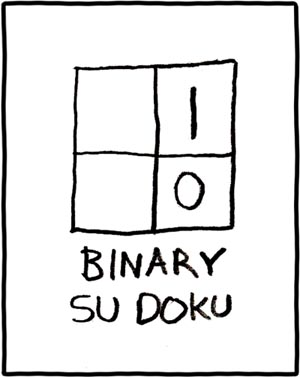
\includegraphics[totalheight=6cm]{bilder/XKCD/su_doku}
	
	\subsubsection{Schlüsselqualifikationen / Mathe-Wahl\-pflicht}
	Hier können überfachliche Veranstaltungen aus dem Schlüsselqualifikations-Pool eingebracht werden. Da das ca. 100 angebotene Verstanstaltungen pro Semester sind, findest du sie nicht im Modulhandbuch oder im Informatik-Studenplan, sondern im QIS\footnote{\verUrl{2}{https://vorlesungen.tu-bs.de/qisserver/rds?state=wtree\&search=1\&trex=step\&root120152=99799|103438\&P.vx=kurz}}. Daneben ist es möglich Veranstaltungen der \textit{Trainings handlungsbezogener Kompetenzen des Lehrstuhls für Arbeits-, Organisations- und Sozialpsychologie} einzubringen\footnote{\verUrl{1}{https://www.tu-braunschweig.de/psychologie/abt/aos/studiumlehre/hbk}} oder des Sprachzentrums (siehe unten). 
	Außerdem können vier Credits im Rahmen des \textit{SCOUT-Programm des Instituts für Arbeits- , Organisations- und Sozialpsychologie} eingebracht werden. Hier werden internationale Studierende von dir als SCOUT ein Semester lang begleitet, um ihnen die Integration in den deutschen Unialltag zu erleichtern\footnote{\verUrl{1}{https://www.tu-braunschweig.de/scout}}. Zu beachten ist, dass man dabei nur Fächer belegen darf, die nicht aus seinem Nebenfach stammen. Man kann also z.B mit den Nebenfach Mathe nicht Schlüsselqualifikationen der Mathematik belegen. Soweit die Regelungen für beide Studiengänge, nun die spezifischen:

	\paragraph*{Schlüsselqualifikationen im Bachelor}
	Im Bachelor musst du zehn Credits in Schlüsselqualifikationen belegen, die du dir nahezu beliebig aussuchen darfst. Das Modul besteht aus mehreren unbenoteten Studienleistungen. Dies gilt auch dann, wenn du einen benoteten Schein bekommst.\\
	Außerdem musst du zehn Credits im Wahlpflichtbereich Mathematik erbringen. Die Auswahl besteht zur Zeit aus drei Fächern, eins im Winter und eins im Sommer. Die beiden Wahlpflichtfächer Mathe gehen benotet ein.

	\paragraph*{Schlüsselqualifikationen im Master}
	Im Master kannst du acht bis zehn Credits als Schlüsselqualifikation belegen. Es gibt ansonsten nur einen Unterschied zur Bachelorregelung: Sofern du nicht gerade Mathe als Nebenfach belegst, kannst du dort auch Mathewahlpflichtfächer einbringen. Der Master hat sonst keinen Mathewahlpflichtbereich. Auch im Master besteht der Schlüsselqualifikationenblock aus unbenoteten Studienleistungen.

	\subsubsection{Sprachenzentrum}
	Am Sprachenzentrum der Uni kannst du verschiedene Sprachkurse belegen, die auch als Schlüsselqualifikationen zählen (maximal 8 Credits). Auf den Seiten des Sprachenzentrums (\verUrl{1}{https://www.tu-braunschweig.de/sprachenzentrum}) findest du alle angebotenen Kurse. Um sich für Kurse anzumelden, brauchst du ein Konto, das du persönlich in der Mediothek (im Altgebäude \verUrl{1}{https://www.tu-braunschweig.de/sprachenzentrum/beratung/mediothek}) registrieren musst.

	\textbf{Wichtig:} Die Anmeldung für Sprachkurse beginnt bereits in den Semesterferien. Um Plätze zu bekommen, solltest du dich also so früh wie möglich anmelden. Bevor du an einem Englischkurs teilnehmen kannst, musst du zunächst einen Einstufungstest machen. Die Termine findest du hier: \verUrl{1}{https://www.tu-braunschweig.de/sprachenzentrum/sprachen/einstufungstests}\\ 
	Da gerade bei diesen Kursen die Nachfrage sehr hoch ist, solltest du den Test möglichst bereits vor dem Anmeldungszeitraum (beginnt etwa 2 Wochen vor Vorlesungsbeginn) ablegen.

	\subsubsection{Praktikum}
	Teilweise werden auf Vorlesungen aufbauende Praktika angeboten, die das erworbene Wissen praktisch vertiefen sollen. Der Ablauf sieht so aus, dass man bestimmte Aufgaben lösen und die Lösung abgeben muss. Anschließend sind die Ergebnise einem Übungsleiter vorzuführen und zu erklären. Es kann sich dabei um einzelne Teilaufgaben oder ein großes Softwareprojekt handeln, ähnlich dem SEP oder Teamprojekt. Im Regelfall handelt es sich bei Praktika um unbenotete Studienleistungen.

Es werden folgende	Arten von Praktika unterschieden:
	
	\begin{itemize}
		\item Es gibt Veranstaltungen, bei denen die Teilnahme am Praktikum verpflichtend ist, um den Schein zur Vorlesung zu bekommen. 
		\item Es gibt freiwillige Praktika als Alternative oder Ergänzung zur Vorlesung.
		\item Außerdem gibt es Prakika, bei denen man sich aussuchen kann, ob man sie als Teil einer Vorlesung (so genannte Supermodule) oder als eigenes Modul belegen möchte.
	\end{itemize}

\noindent	Die Menge der Praktika, die du in das Studium einbringst, wird u.a. dadurch beschränkt, wie viele unbenotete Studienleistungen du einbringen darfst, bzw. umgekehrt darüber, wie viele benotete Leistungen erwartet werden.

	\subsubsection*{SEP (Software-Entwicklungs-Praktikum)}
	Eine Sonderform des Praktikums ist das SEP im Bachelor. Es wird üblicherweise im 4. Semester (Studienbeginn WS) oder 5. Semester (Studienbeginn SS) absolviert. Von normalen Praktika unterscheidet es sich dadurch, dass es verpflichtend ist. Es geht darum, im Team das \textbf{gelernte Wissen} aus den Vorlesungen \emph{Programmieren 1+2}, sowie \emph{Software Engeneering 1} anzuwenden, indem man ein Softwareprojekt (Entwicklung und Dokumentation) umsetzt. Das SEP ist eine unbenotete Studienleistung.

	\subsubsection*{Teamprojekt}
	Ebenfalls ein spezielles Praktikum ist das Teamprojekt. Es verfolgt eine ähnliche Zielsetzung wie das SEP mit dem Unterschied, dass es weniger formale Vorgaben gibt und man sich selbst ein Thema suchen kann. Dazu empfiehlt es sich, rechtzeitig auf den Webseiten der Institute nachzuschauen und sich eine Gruppe zu suchen. Wie das SEP ist auch das Teamprojekt eine Studienleistung.

	\subsubsection{Projektarbeit im Master}
	Für den Master kommt noch die Projektarbeit hinzu. Dies ist eine
	freiwillige Prüfungsleistungsleistung, die aus einem eigenständig
	bearbeiteten Projekt mit schriftlicher Ausarbeitung besteht. Das Modul umfasst 15 Credits.

	\subsubsection{Abschlussarbeit}
	Die Abschlussarbeit sind 15 Credits im Bachelor und 30 Credits im Master. Dabei geht es darum, dass im Studium erworbene Wissen an einer gegebenen Aufgabenstellung anzuwenden und  die Ergebnisse in einer schriftliche Ausarbeitung festzuhalten. Wie beim Teamprojekt gilt auch hier, dass die Institute oft Themen vorschlagen.  Man kann auch ein eigenes Thema vorschlagen, wenn es ins Forschungsprofil des Institus passt. \textbf{Wichtig:} Bevor du die Abschlussarbeit anmelden kannst, musst du bestimmte Vorraussetzungen erfüllen:
	\begin{itemize}
		\item Bachelorarbeit: Sämtliche Pflichtfächer (Grundlagen der Informatik, Mathematik und Informatik der Systeme).
		\item Masterarbeit: Module im Umfang von 75 Credits müssen vor Anmeldung absolviert worden sein.
	\end{itemize}

%%% Local Variables: 
%%% mode: latex
%%% TeX-master: "../../1-te_ws"
%%% End: 
